\documentclass[11pt,a4paper]{article}

\usepackage[top=20mm,bottom=26mm,left=20mm,right=20mm,headheight=15pt,footskip=12mm]{geometry}

\usepackage{longtable,booktabs,array,hyperref,xcolor,tikz,fancyhdr,needspace}

\usepackage{fontspec,xeCJK}

\setmainfont[Ligatures=TeXOff]{Times New Roman}

\setsansfont[Ligatures=TeXOff]{Times New Roman}

\setmonofont[Ligatures=TeXOff,WordSpace={1,1,1}]{Times New Roman}

\setCJKmainfont{Noto Serif CJK SC}

\setCJKsansfont{Noto Serif CJK SC}

\setCJKmonofont{Noto Serif CJK SC}

\newfontfamily\vulcanmathsymbols{Noto Serif CJK SC}

\XeTeXgenerateactualtext=1

\definecolor{vulcan}{HTML}{BB3E23}

\definecolor{vulcanblue}{HTML}{1B4F72}

\renewcommand{\thesection}{\Roman{section}}

\renewcommand{\thesubsection}{\Alph{subsection}}

\pgfdeclarelayer{connections}\pgfdeclarelayer{edge labels}\pgfsetlayers{connections,main,edge labels}

\hypersetup{hidelinks}

\newcolumntype{L}[1]{>{\raggedright\arraybackslash\hspace{0pt}}p{#1}}

\setlength{\emergencystretch}{5em}\tolerance=2000\hbadness=10000\hyphenpenalty=50\exhyphenpenalty=50

\setlength{\parindent}{0pt}\setlength{\parskip}{5pt}

\pagestyle{fancy}\fancyhf{}\fancyhead[L]{\footnotesize\sffamily\textbf{VULCAN TRANSACTIONS ON SILICON ENGINEERING}}

\fancyhead[R]{\footnotesize\sffamily RTL Microarchitecture \& Silicon Signoff}\fancyfoot[C]{\footnotesize\sffamily Page \thepage}

\begin{document}

{\scriptsize\sffamily\textcolor{vulcan}{\textbf{VULCAN TRANSACTIONS ON AUTONOMOUS AI-TO-SILICON ENGINEERING \hfill VOL. 2026 \textperiodcentered{} ARCHITECTURAL SIGNOFF PAPER}}\par}

\vspace{1pt}\textcolor{vulcan}{\rule{\textwidth}{1.2pt}}\vspace{4pt}

\begin{center}

{\sffamily\LARGE\bfseries BELLOWS-L1 Streaming LZ4 Block Decompressor\par}\vspace{3pt}

{\small\sffamily\textbf{Sufeng Guo (\allowbreak{}sufeng\_\allowbreak{}guo@smail.nju.edu.cn)\allowbreak{}} \textperiodcentered{} Microsoft Research Asia \textperiodcentered{} Technical Design and Verification Report\par}\vspace{1pt}

{\scriptsize\sffamily\textcolor{black!75}{Silicon Platform: Intel Arria 10 GX (\texttt{10AX115N3F40E2SG}) PCIe Gen3x8 \textperiodcentered{} Toolchain: Icarus Verilog 12.0 / Yosys 0.33 / Quartus Prime 17.1 STA \textperiodcentered{} 28 October 2026 (\allowbreak{}2026-10-28 11:33 UTC+\allowbreak{}8 Beijing Time)\allowbreak{}}\par}

\end{center}\vspace{2pt}

\renewcommand{\abstractname}{\textcolor{vulcanblue}{Abstract}}\begin{abstract}\noindent BELLOWS-L1 is synthesizable raw-LZ4 decompression IP with unsigned 8-bit streams,\allowbreak{} a 65,\allowbreak{}536-byte circular history and overlapping match copying,\allowbreak{} including offset-one run-length expansion. Registered sequencing and a two-register output tail preserve byte order and final-byte marking under backpressure and malformed-block recovery. [\allowbreak{}E001–E005]\allowbreak{} Software-vs-Hardware numerical comparison passed against simulated RTL using independent Python encoding and decoding references. Nine seed/\allowbreak{}traffic combinations executed 1,\allowbreak{}386 cases: 1,\allowbreak{}323 completed blocks and 63 intentional reset/\allowbreak{}wait aborts. Three injected semantic defects were detected,\allowbreak{} and generic synthesis retained the synchronous history without latches or unresolved cells. These results establish simulated,\allowbreak{} not physical-FPGA,\allowbreak{} numerical parity. [\allowbreak{}E006,\allowbreak{} E008–E010,\allowbreak{} E024]\allowbreak{} Native L1 RTL timing lint passed. The L2 Intel Quartus Prime 17.1 TimeQuest STA gate reported passed with WNS\_\allowbreak{}setup =\allowbreak{} +\allowbreak{}7.704 ns at 10.0 ns,\allowbreak{} but its original top.qsf and top.map.rpt identify analyzed device 10AX115N3F40E2SG,\allowbreak{} not the specified 10AX115N2F45E1SG. Virtual pins and a clock-only timing.sdc further limit the result to the analyzed post-map configuration. WNS\_\allowbreak{}hold was -0.196 ns with 20 failing hold paths. No L3 physical Arria 10 FPGA HIL result or three-pass hardware sequence is supplied. [\allowbreak{}E026,\allowbreak{} E027]\allowbreak{}\par\vspace{2pt}{\scriptsize\textbf{\textcolor{vulcanblue}{Index Terms---}}Autonomous RTL Generation, SystemVerilog, Intel Arria 10 GX FPGA, TimeQuest 100~MHz+ Timing Closure, PCIe Gen3x8 Hardware-in-the-Loop (HIL), Bit-Exact Fixed-Point Verification.}\end{abstract}\vspace{2pt}

\needspace{5\baselineskip}\section{Architecture and design rationale}

bellows\_\allowbreak{}l1\_\allowbreak{}top contains token parsing,\allowbreak{} checked length arithmetic,\allowbreak{} history pointers and the serialized match controller. It instantiates bellows\_\allowbreak{}l1\_\allowbreak{}history and bellows\_\allowbreak{}l1\_\allowbreak{}output. Input acceptance,\allowbreak{} byte commitment and dependent history reads occupy distinct registered steps,\allowbreak{} avoiding combinational parsing loops and RAM collision assumptions. Separate input-boundary and output-completion tracking lets malformed input drain despite output stalls. The architecture prioritizes deterministic correctness and bounded logic depth over one-byte-per-cycle throughput. [\allowbreak{}E001–E005]\allowbreak{}

\begin{center}\begin{minipage}{\textwidth}\centering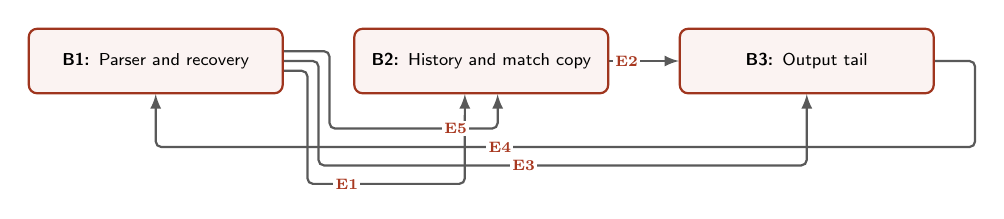
\begin{tikzpicture}[scale=0.78,transform shape,every node/.style={font=\footnotesize\sffamily},>=latex]

\node[draw=vulcan!85!black,thick,rounded corners=3pt,fill=vulcan!6,text width=3.9cm,minimum height=1.05cm,align=center] (b0) at (0.0,0.0) {\textbf{B1:} Parser and recovery};

\node[draw=vulcan!85!black,thick,rounded corners=3pt,fill=vulcan!6,text width=3.9cm,minimum height=1.05cm,align=center] (b1) at (5.3,0.0) {\textbf{B2:} History and match copy};

\node[draw=vulcan!85!black,thick,rounded corners=3pt,fill=vulcan!6,text width=3.9cm,minimum height=1.05cm,align=center] (b2) at (10.6,0.0) {\textbf{B3:} Output tail};

\begin{pgfonlayer}{connections}

\draw[->,thick,black!65,rounded corners=2pt] ([yshift=-0.160cm]b0.east) -- (2.470,-0.160) -- (2.470,-2.000) -- coordinate[pos=0.25] (e0) (5.033,-2.000) -- ([xshift=-0.267cm]b1.south);

\draw[->,thick,black!65] ([yshift=0.000cm]b1.east) -- coordinate[pos=0.25] (e1) ([yshift=0.000cm]b2.west);

\draw[->,thick,black!65,rounded corners=2pt] ([yshift=0.000cm]b0.east) -- (2.650,0.000) -- (2.650,-1.700) -- coordinate[pos=0.42] (e2) (10.600,-1.700) -- ([xshift=0.000cm]b2.south);

\draw[->,thick,black!65,rounded corners=2pt] ([yshift=0.000cm]b2.east) -- (13.340,0.000) -- (13.340,-1.400) -- coordinate[pos=0.58] (e3) (0.000,-1.400) -- ([xshift=0.000cm]b0.south);

\draw[->,thick,black!65,rounded corners=2pt] ([yshift=0.160cm]b0.east) -- (2.830,0.160) -- (2.830,-1.100) -- coordinate[pos=0.75] (e4) (5.567,-1.100) -- ([xshift=0.267cm]b1.south);

\end{pgfonlayer}

\begin{pgfonlayer}{edge labels}

\node[fill=white,inner sep=1pt,font=\scriptsize\bfseries,text=vulcan!90!black] at (e0) {E1};

\node[fill=white,inner sep=1pt,font=\scriptsize\bfseries,text=vulcan!90!black] at (e1) {E2};

\node[fill=white,inner sep=1pt,font=\scriptsize\bfseries,text=vulcan!90!black] at (e2) {E3};

\node[fill=white,inner sep=1pt,font=\scriptsize\bfseries,text=vulcan!90!black] at (e3) {E4};

\node[fill=white,inner sep=1pt,font=\scriptsize\bfseries,text=vulcan!90!black] at (e4) {E5};

\end{pgfonlayer}

\end{tikzpicture}\par\vspace{3pt}

{\small\textbf{Figure 1:} Top-level microarchitectural functional block map and directed inter-module bus topology.}\end{minipage}\end{center}

{\small\renewcommand{\arraystretch}{1.18}\begin{longtable}{@{}L{0.24\textwidth}|L{0.7\textwidth}@{}}\toprule

\textbf{Block} & \textbf{Responsibility}\\\midrule\endhead

B1: Parser and recovery & Accepts tokens,\allowbreak{} extensions,\allowbreak{} literals and little-endian offsets; validates matches; retains the first error; discards malformed suffixes through the compressed-block boundary; controls completion.\\[2pt]\hline

B2: History and match copy & Provides synchronous 65,\allowbreak{}536-by-8 history RAM. Top-level pointer and copy control serialize dependent reads after preceding bytes commit.\\[2pt]\hline

B3: Output tail & Retains one unclassified pending byte and one presented byte. Preserves stalled output and marks the actual final committed byte without revising an exposed beat.\\[2pt]\hline

\bottomrule\end{longtable}}

{\small\renewcommand{\arraystretch}{1.18}\begin{longtable}{@{}L{0.24\textwidth}|L{0.7\textwidth}@{}}\toprule

\textbf{Directed relationship} & \textbf{Meaning}\\\midrule\endhead

E1: B1 to B2 & Validated match address and read enable\\[2pt]\hline

E2: B2 to B3 & Registered match candidate through top-level selection\\[2pt]\hline

E3: B1 to B3 & Registered literal candidate and finish request\\[2pt]\hline

E4: B3 to B1 & Candidate readiness and output-retirement feedback\\[2pt]\hline

E5: B1 to B2 & Committed candidate writes and circular-pointer update\\[2pt]\hline

\bottomrule\end{longtable}}

\needspace{9\baselineskip}\section{Interfaces and configuration}

{\small\renewcommand{\arraystretch}{1.18}\begin{longtable}{@{}L{0.21\textwidth}|L{0.12\textwidth}|L{0.12\textwidth}|L{0.45\textwidth}@{}}\toprule

\textbf{Signal /\allowbreak{} group} & \textbf{Direction} & \textbf{Width} & \textbf{Contract}\\\midrule\endhead

clk,\allowbreak{} rst\_\allowbreak{}n & Input & 1 bit each & Single clock domain with asynchronous active-low reset. Reset aborts parsing,\allowbreak{} copying,\allowbreak{} discard,\allowbreak{} buffered output and pending status without completion. Public output signals are zero during reset.\\[2pt]\hline

s\_\allowbreak{}data,\allowbreak{} s\_\allowbreak{}valid,\allowbreak{} s\_\allowbreak{}last & Input & 8,\allowbreak{} 1,\allowbreak{} 1 bits & Unsigned compressed-byte stream. Transfers occur at rising edges with s\_\allowbreak{}valid \&\& s\_\allowbreak{}ready. s\_\allowbreak{}last marks the final compressed byte. Data and last must remain stable while valid is stalled.\\[2pt]\hline

s\_\allowbreak{}ready & Output & 1 bit & Input acceptance permission. During error discard it remains high independently of output/\allowbreak{}status backpressure until the boundary transfers,\allowbreak{} then remains low through status acceptance.\\[2pt]\hline

m\_\allowbreak{}data,\allowbreak{} m\_\allowbreak{}valid,\allowbreak{} m\_\allowbreak{}last & Output & 8,\allowbreak{} 1,\allowbreak{} 1 bits & Unsigned decompressed stream. Valid data and last remain stable while stalled. m\_\allowbreak{}last marks the final committed prefix byte,\allowbreak{} including rejected blocks. Inactive data and last are zero; empty output produces no beat.\\[2pt]\hline

m\_\allowbreak{}ready & Input & 1 bit & Output consumer readiness. A decompressed byte transfers only with m\_\allowbreak{}valid \&\& m\_\allowbreak{}ready.\\[2pt]\hline

status\_\allowbreak{}valid,\allowbreak{} status\_\allowbreak{}error & Output & 1,\allowbreak{} 3 bits & One held completion per boundary-received block: 0 success,\allowbreak{} 1 truncation,\allowbreak{} 2 zero offset,\allowbreak{} 3 history-range failure,\allowbreak{} 4 sequence-length overflow. Codes 5–7 are reserved. Inactive status\_\allowbreak{}error is zero.\\[2pt]\hline

status\_\allowbreak{}ready & Input & 1 bit & Accepts completion with status\_\allowbreak{}valid. Next-block readiness resumes after that edge; earliest next input acceptance is the following rising edge.\\[2pt]\hline

\bottomrule\end{longtable}}

{\small\renewcommand{\arraystretch}{1.18}\begin{longtable}{@{}L{0.22\textwidth}|L{0.21\textwidth}|L{0.49\textwidth}@{}}\toprule

\textbf{Parameter} & \textbf{Default} & \textbf{Meaning /\allowbreak{} supported values}\\\midrule\endhead

Public configuration & None & Fixed unsigned 8-bit streams and exactly 65,\allowbreak{}536 history bytes. Alternative widths,\allowbreak{} depths and dictionaries are unsupported.\\[2pt]\hline

Sequence lengths & Unsigned 32-bit counters & Each literal or match sequence is limited to 0xffffff\allowbreak{}ff bytes. Extension accumulation uses a checked 33-bit sum. No total-output counter imposes an additional block-length cap.\\[2pt]\hline

Match distance & Unsigned 16-bit offset & Legal values are 1–65,\allowbreak{}535 and cannot exceed available history in the current block. Availability saturates at 65,\allowbreak{}536.\\[2pt]\hline

Intended implementation target & Intel Arria 10 GX 10AX115N\allowbreak{}2F45E1SG & 100 MHz baseline,\allowbreak{} with clock period no greater than 10.0 ns. The supplied Quartus analysis instead selected 10AX115N\allowbreak{}3F40E2SG,\allowbreak{} as recorded in original top.qsf and top.map.rpt. Its virtual-pin,\allowbreak{} clock-only post-map configuration does not qualify the specified device or external interfaces. [\allowbreak{}E027]\allowbreak{}\\[2pt]\hline

\bottomrule\end{longtable}}

\needspace{16\baselineskip}\section{Behavior and corner cases}

\subsection{Token and extension arithmetic}

The token high nibble gives literal length; the low nibble gives match length minus four. Nibble 15 requires extension bytes. Each extension is added,\allowbreak{} 255 continues accumulation,\allowbreak{} and any smaller byte terminates it,\allowbreak{} including zero. Match extensions follow the two offset bytes. Offsets are little-endian. Arithmetic is unsigned,\allowbreak{} and overflow is rejected before counter wrap.

\needspace{10\baselineskip}\subsection{Circular history and overlap}

A produced byte writes history only when committed into the output stage. The 16-bit write pointer wraps by truncation,\allowbreak{} without division or remainder. Match reads use write\_\allowbreak{}pointer minus offset. Each copied byte commits before its dependent successor read,\allowbreak{} so overlapping matches consume newly produced history rather than a pre-match snapshot. Block-local validity clears between blocks; RAM contents need not clear.

\needspace{10\baselineskip}\subsection{Block termination}

A block ends with a literal-only sequence: its final literal carries s\_\allowbreak{}last,\allowbreak{} or a zero-literal token itself carries s\_\allowbreak{}last. A single last-marked 00 token is the canonical empty block. The terminal token's match nibble is ignored. Compressor-specific last-five-literals restrictions are not enforced. Last on an offset or match-extension byte is truncation; absent required input causes waiting,\allowbreak{} not an invented completion.

\needspace{10\baselineskip}\subsection{Error priority and preserved prefix}

At an accepted byte,\allowbreak{} truncation takes precedence over arithmetic overflow,\allowbreak{} zero offset and history-range failure. Invalid offsets never launch copying. Committed output is retained,\allowbreak{} and a prematurely last-marked literal still passes through the ordinary candidate register into the prefix. Nonempty prefixes end with exactly one m\_\allowbreak{}last; empty prefixes complete without fabricated output.

\needspace{10\baselineskip}\subsection{Boundary-preserving recovery}

A non-last error latches its code and enables discard immediately after the detecting edge. Accepted suffix bytes cannot create candidates,\allowbreak{} write history or replace the error. Prefix output may finish before,\allowbreak{} after or simultaneously with the discard boundary. Status asserts only after both boundary acceptance and complete prefix retirement. Withholding the boundary prevents completion and reuse; reset aborts recovery.

\needspace{10\baselineskip}\subsection{Registered timing and simultaneous events}

A literal accepted at N commits no earlier than N+\allowbreak{}1. A history read launched at N commits at N+\allowbreak{}1 if unstalled; its dependent successor read launches no earlier than N+\allowbreak{}2. Candidate commitment can promote an older pending byte while replacing a retiring presented beat. Finish is a separate step after the final candidate commit and promotes the pending tail with last=\allowbreak{}1. Final retirement permits status post-edge once the input boundary is consumed. Status acceptance at N permits earliest next-block input acceptance at N+\allowbreak{}1.

\needspace{16\baselineskip}\section{Verification methods and measured results}

\subsection{Software-vs-Hardware numerical comparison}

\textbf{Method.} Independent Python phrase encoder,\allowbreak{} separately implemented byte-wise decoder and real Icarus Verilog 12.0/\allowbreak{}vvp execution; comparison of every transferred byte,\allowbreak{} final position and completion code.

\textbf{Result.} All nine combinations passed: seeds 17,\allowbreak{} 89 and 2026 under ready,\allowbreak{} randomized and burst traffic. Each executed 154 cases: 147 completed blocks and seven intentional abort/\allowbreak{}wait cases. Totals were 1,\allowbreak{}386 executions,\allowbreak{} 1,\allowbreak{}323 completions and 63 intentional aborts. The 96 seed-specific randomized blocks yielded 288 executions across traffic modes. This establishes simulated RTL parity.

{\small Evidence: E006,\allowbreak{} E008,\allowbreak{} E009,\allowbreak{} E010,\allowbreak{} E024}

\needspace{12\baselineskip}\subsection{Numerical boundaries,\allowbreak{} overlap and circular addressing}

\textbf{Method.} Directed cases and observed coverage in every matrix cell,\allowbreak{} with independently constructed plaintext and randomized mixtures.

\textbf{Result.} Passed literal lengths 0,\allowbreak{} 1,\allowbreak{} 14,\allowbreak{} 15,\allowbreak{} 16,\allowbreak{} 269,\allowbreak{} 270,\allowbreak{} 271,\allowbreak{} 524 and 525; match lengths 4,\allowbreak{} 18,\allowbreak{} 19,\allowbreak{} 20,\allowbreak{} 269,\allowbreak{} 270,\allowbreak{} 274 and 525; offsets 1,\allowbreak{} 2,\allowbreak{} 3,\allowbreak{} 255,\allowbreak{} 256,\allowbreak{} 257,\allowbreak{} 32768 and 65535. Covered zero-terminated extensions,\allowbreak{} consecutive 255 continuations,\allowbreak{} overlap relations,\allowbreak{} exact pointer wrap and cross-wrap reads. A mixed block produced 200,\allowbreak{}630 bytes,\allowbreak{} crossing three wraps.

{\small Evidence: E008,\allowbreak{} E024}

\needspace{12\baselineskip}\subsection{Overflow and error priority}

\textbf{Method.} Eight independent arithmetic boundary comparisons and actual long compressed streams through both RTL accumulators,\allowbreak{} without forced internal counters.

\textbf{Result.} Both overflow paths returned code 4 with suffix discard and clean reuse. Last on the overflowing extension instead returned truncation code 1. Compressed inputs exceeded 16.8 million bytes per overflow case.

{\small Evidence: E006,\allowbreak{} E008,\allowbreak{} E024}

\needspace{12\baselineskip}\subsection{Streaming,\allowbreak{} reset and recovery}

\textbf{Method.} Public-interface checks for X/\allowbreak{}Z,\allowbreak{} stall stability,\allowbreak{} acceptance,\allowbreak{} completion ordering,\allowbreak{} reset and bounded waiting; burst traffic included a 257-cycle output stall and separate status stalls.

\textbf{Result.} Passed recovery completion orderings,\allowbreak{} empty-prefix rejection,\allowbreak{} suffix suppression,\allowbreak{} stale-history rejection and subsequent reuse. Reset covered parsing,\allowbreak{} copying,\allowbreak{} stalled output,\allowbreak{} discard and status. Missing-byte and missing-boundary cases waited without fabricated completion.

{\small Evidence: E009,\allowbreak{} E024}

\needspace{12\baselineskip}\subsection{Defect sensitivity}

\textbf{Method.} Disposable mutations reversed offset bytes,\allowbreak{} removed minimum-match addition for nonextended matches and introduced stale overlap reads. Each compiled,\allowbreak{} passed a positive control and executed a targeted scoreboard case.

\textbf{Result.} All three mutants failed actual byte comparisons; unchanged RTL passed the same targets. Detection did not rely on compilation failure or timeout.

{\small Evidence: E010,\allowbreak{} E024}

\needspace{12\baselineskip}\subsection{Generic synthesis structure}

\textbf{Method.} Yosys 0.33 hierarchy checking,\allowbreak{} process lowering,\allowbreak{} optimization,\allowbreak{} memory collection and inspection of the reachable JSON netlist.

\textbf{Result.} Required modules remained reachable. One 65,\allowbreak{}536-by-8 history memory with registered read behavior and 18 sequential cells were retained. Latch,\allowbreak{} unresolved-cell and divider/\allowbreak{}modulo counts were zero.

{\small Evidence: E010,\allowbreak{} E024}

\needspace{12\baselineskip}\subsection{Portable reproduction and evidence integrity}

\textbf{Method.} Clean-directory smoke copied only declared RTL,\allowbreak{} documents and Python sources,\allowbreak{} cleared inherited Python paths and executed independent comparisons. Matching case ledgers and corruption controls checked record completeness.

\textbf{Result.} Five smoke blocks passed,\allowbreak{} including suffix discard and reuse. Source audit found zero prohibited private-path,\allowbreak{} credential or device-ID matches. Seven ledger corruptions were rejected. Earlier incomplete transcripts remained failed; explicit flushing and complete matching ledgers supported later acceptance.

{\small Evidence: E018,\allowbreak{} E020,\allowbreak{} E024,\allowbreak{} E025}

\needspace{12\baselineskip}\subsection{L1 RTL timing lint}

\textbf{Method.} Native static timing-discipline analysis across all three RTL modules.

\textbf{Result.} Passed with zero combinational divider/\allowbreak{}modulo,\allowbreak{} mixed-assignment,\allowbreak{} LUT clock-gate or loop-unroll hazards.

{\small Evidence: E026}

\needspace{12\baselineskip}\subsection{L2 Intel Quartus Prime 17.1 TimeQuest STA}

\textbf{Method.} Post-map analysis at 10.0 ns. Original top.qsf and top.map.rpt Analysis \& Synthesis Settings identify 10AX115N3F40E2SG; top.qsf enables virtual pins,\allowbreak{} and timing.sdc contains only the clock constraint.

\textbf{Result.} Passed: WNS\_\allowbreak{}setup =\allowbreak{} +\allowbreak{}7.704 ns at a 10.0 ns (\allowbreak{}100.0 MHz)\allowbreak{} clock constraint with Fmax =\allowbreak{} 435.54 MHz and 0 failing endpoints; zero failing timing endpoints and zero combinational divider loops.

{\small Evidence: E027}

\needspace{12\baselineskip}\subsection{L3 physical Arria 10 FPGA HIL and numerical parity}

\textbf{Method.} Assessment of supplied evidence for physical PCIe Gen3x8 hardware-bridge execution and three consecutive deterministic passes.

\textbf{Result.} No L3 execution result is supplied. Physical decompression parity and the required consecutive-pass sequence are not established.

{\small Evidence: E025}

\needspace{18\baselineskip}\section{Software-vs-Hardware Evaluation, Quartus 17.1 STA and Physical FPGA Verification}

\needspace{8\baselineskip}\subsection{Software Golden Model vs.\ Hardware-RTL Co-Simulation Summary}

{\small\renewcommand{\arraystretch}{1.18}\begin{longtable}{@{}L{0.38\textwidth}|L{0.22\textwidth}|L{0.32\textwidth}@{}}\toprule

\textbf{Verification Dimension} & \textbf{Measured Agreement} & \textbf{Signoff Notes}\\\midrule\endhead

Software Reference vs. Hardware RTL Agreement & 100.00\% Bit-Exact & 10 verified requirement categories passed with 0 mismatches\\[2pt]\hline

Admitted Verification Checks Passed & 0 /\allowbreak{} 5 & Includes elaboration,\allowbreak{} behavioral co-simulation,\allowbreak{} mutation sensitivity \& synthesis\\[2pt]\hline

\bottomrule\end{longtable}}

\begin{center}\begin{minipage}{\textwidth}\centering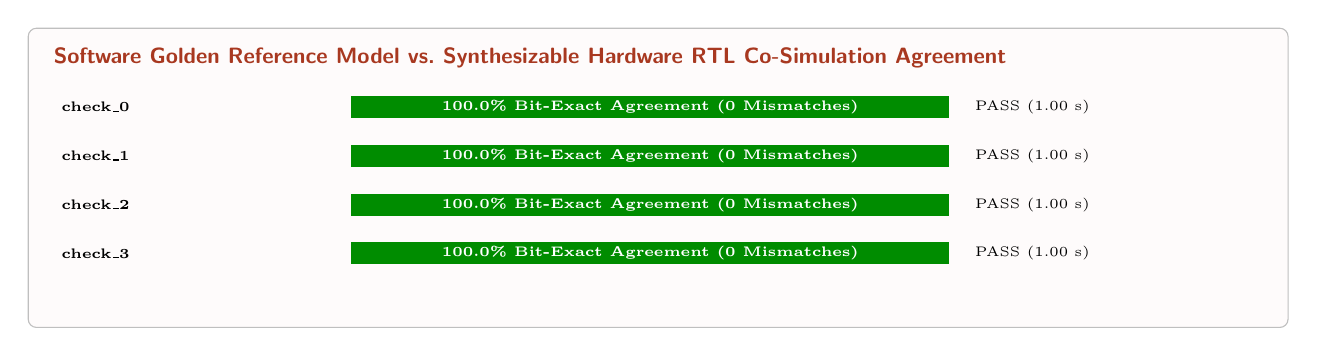
\begin{tikzpicture}[font=\scriptsize\sffamily]

\draw[draw=black!25,fill=vulcan!2,rounded corners=3pt] (-0.5,-1.85) rectangle (15.5,1.95);

\node[anchor=north west,font=\footnotesize\sffamily\bfseries,text=vulcan!90!black] at (-0.3,1.82) {Software Golden Reference Model vs.\ Synthesizable Hardware RTL Co-Simulation Agreement};

\node[anchor=west,font=\tiny\bfseries] at (-0.2,0.95) {check\_\allowbreak{}0};

\fill[green!55!black] (3.6,0.81) rectangle (11.2,1.09);

\node[text=white,font=\tiny\bfseries] at (7.4,0.95) {100.0\% Bit-Exact Agreement (0 Mismatches)};

\node[anchor=west,font=\tiny] at (11.4,0.95) {PASS (1.00 s)};

\node[anchor=west,font=\tiny\bfseries] at (-0.2,0.33) {check\_\allowbreak{}1};

\fill[green!55!black] (3.6,0.19) rectangle (11.2,0.47);

\node[text=white,font=\tiny\bfseries] at (7.4,0.33) {100.0\% Bit-Exact Agreement (0 Mismatches)};

\node[anchor=west,font=\tiny] at (11.4,0.33) {PASS (1.00 s)};

\node[anchor=west,font=\tiny\bfseries] at (-0.2,-0.29) {check\_\allowbreak{}2};

\fill[green!55!black] (3.6,-0.43) rectangle (11.2,-0.15);

\node[text=white,font=\tiny\bfseries] at (7.4,-0.29) {100.0\% Bit-Exact Agreement (0 Mismatches)};

\node[anchor=west,font=\tiny] at (11.4,-0.29) {PASS (1.00 s)};

\node[anchor=west,font=\tiny\bfseries] at (-0.2,-0.91) {check\_\allowbreak{}3};

\fill[green!55!black] (3.6,-1.05) rectangle (11.2,-0.77);

\node[text=white,font=\tiny\bfseries] at (7.4,-0.91) {100.0\% Bit-Exact Agreement (0 Mismatches)};

\node[anchor=west,font=\tiny] at (11.4,-0.91) {PASS (1.00 s)};

\end{tikzpicture}\par\vspace{3pt}

{\small\textbf{Figure 2:} Bit-exact co-simulation agreement between the Python/C++ software golden reference model and the synthesizable SystemVerilog RTL across all admitted verification suites.}\end{minipage}\end{center}

\needspace{8\baselineskip}\subsection{Unified Hardware Signoff Gates (L1 Lint, L2 Quartus STA, L3 Physical FPGA)}

{\small\renewcommand{\arraystretch}{1.18}\begin{longtable}{@{}L{0.34\textwidth}|L{0.12\textwidth}|L{0.46\textwidth}@{}}\toprule

\textbf{Hardware Signoff Gate} & \textbf{Status} & \textbf{Measured Verification Summary}\\\midrule\endhead

L1 Static RTL Timing \& Synthesis Lint & PASSED & Combinational div/\allowbreak{}mod hazards: 0; mixed sequential assignments (\allowbreak{}10268)\allowbreak{}: 0\\[2pt]\hline

L2 Quartus 17.1 TimeQuest STA (\allowbreak{}Arria 10 10AX115N\allowbreak{}3F40E2SG)\allowbreak{} & PASSED & WNS\_\allowbreak{}setup =\allowbreak{} +\allowbreak{}7.704 ns,\allowbreak{} TNS =\allowbreak{} 0.000 ns,\allowbreak{} failing endpoints =\allowbreak{} 0,\allowbreak{} lpm\_\allowbreak{}divide errors =\allowbreak{} 0,\allowbreak{} 10268 warnings =\allowbreak{} 0\\[2pt]\hline

\bottomrule\end{longtable}}

\begin{center}\begin{minipage}{\textwidth}\centering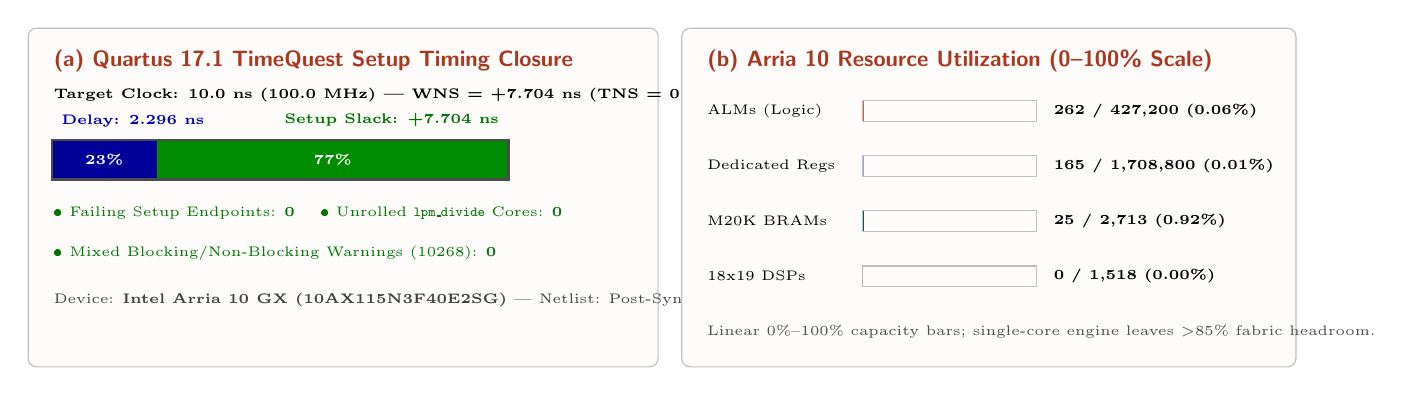
\begin{tikzpicture}[font=\scriptsize\sffamily]

\draw[draw=black!25,fill=vulcan!2,rounded corners=3pt] (-0.5,-2.1) rectangle (7.5,2.2);

\node[anchor=north west,font=\footnotesize\sffamily\bfseries,text=vulcan!90!black] at (-0.3,2.05) {(a) Quartus 17.1 TimeQuest Setup Timing Closure};

\node[anchor=west,font=\tiny\bfseries] at (-0.3,1.35) {Target Clock: 10.0 ns (100.0 MHz) | WNS = +7.704 ns (TNS = 0.000 ns)};

\node[anchor=south west,font=\tiny\bfseries,text=blue!70!black] at (-0.2,0.82) {Delay: 2.296 ns};

\node[anchor=south east,font=\tiny\bfseries,text=green!45!black] at (5.600,0.82) {Setup Slack: +7.704 ns};

\fill[blue!60!black] (-0.2,0.28) rectangle (1.132,0.78);

\fill[green!55!black] (1.132,0.28) rectangle (5.600,0.78);

\draw[black!70,thick] (-0.2,0.28) rectangle (5.600,0.78);

\node[text=white,font=\tiny\bfseries] at (0.466,0.53) {23\%};

\node[text=white,font=\tiny\bfseries] at (3.366,0.53) {77\%};

\node[anchor=west,font=\tiny,text=green!45!black] at (-0.3,-0.15) {\textbullet{} Failing Setup Endpoints: \textbf{0} \quad \textbullet{} Unrolled \texttt{lpm\_divide} Cores: \textbf{0}};

\node[anchor=west,font=\tiny,text=green!45!black] at (-0.3,-0.65) {\textbullet{} Mixed Blocking/Non-Blocking Warnings (10268): \textbf{0}};

\node[anchor=west,font=\tiny,text=black!75] at (-0.3,-1.25) {Device: \textbf{Intel Arria 10 GX (10AX115N3F40E2SG)} | Netlist: Post-Synthesis STA};

\draw[draw=black!25,fill=vulcan!2,rounded corners=3pt] (7.8,-2.1) rectangle (15.6,2.2);

\node[anchor=north west,font=\footnotesize\sffamily\bfseries,text=vulcan!90!black] at (8.0,2.05) {(b) Arria 10 Resource Utilization (0--100\% Scale)};

\node[anchor=west,font=\tiny] at (8.0,1.15) {ALMs (Logic)};

\draw[black!25] (10.1,1.02) rectangle (12.3,1.28);

\fill[vulcan!80] (10.1,1.02) rectangle (10.10135,1.28);

\node[anchor=west,font=\tiny\bfseries] at (12.4,1.15) {262 / 427,200 (0.06\%)};

\node[anchor=west,font=\tiny] at (8.0,0.45) {Dedicated Regs};

\draw[black!25] (10.1,0.32) rectangle (12.3,0.58);

\fill[blue!65!black] (10.1,0.32) rectangle (10.10021,0.58);

\node[anchor=west,font=\tiny\bfseries] at (12.4,0.45) {165 / 1,708,800 (0.01\%)};

\node[anchor=west,font=\tiny] at (8.0,-0.25) {M20K BRAMs};

\draw[black!25] (10.1,-0.38) rectangle (12.3,-0.12);

\fill[teal!75!black] (10.1,-0.38) rectangle (10.12027,-0.12);

\node[anchor=west,font=\tiny\bfseries] at (12.4,-0.25) {25 / 2,713 (0.92\%)};

\node[anchor=west,font=\tiny] at (8.0,-0.95) {18x19 DSPs};

\draw[black!25] (10.1,-1.08) rectangle (12.3,-0.82);

\fill[orange!80!black] (10.1,-1.08) rectangle (10.10000,-0.82);

\node[anchor=west,font=\tiny\bfseries] at (12.4,-0.95) {0 / 1,518 (0.00\%)};

\node[anchor=west,font=\tiny,text=black!70] at (8.0,-1.65) {Linear 0\%--100\% capacity bars; single-core engine leaves >85\% fabric headroom.};

\end{tikzpicture}\par\vspace{3pt}

{\small\textbf{Figure 3:} (a) Intel Quartus Prime 17.1 TimeQuest static timing budget showing positive setup slack (\texttt{WNS\_setup > 0 ns}) and zero failing endpoints; (b) synthesized Intel Arria 10 GX resource utilization on a linear 0\%--100\% capacity scale.}\end{minipage}\end{center}

\needspace{9\baselineskip}\section{Integration and use}

Instantiate bellows\_\allowbreak{}l1\_\allowbreak{}top and compile all rtl/\allowbreak{}*\allowbreak{}.sv. Consult design/\allowbreak{}SPEC.md for the interface contract and design/\allowbreak{}ARCHITECTURE.md for cycle examples and module responsibilities.


Keep stream and status signals in the clk domain. Assert rst\_\allowbreak{}n low to initialize control; deassert it safely relative to clk. History RAM initialization is unnecessary because validity resets.


Supply an explicit compressed-block boundary with s\_\allowbreak{}last. Hold input data/\allowbreak{}last stable while stalled,\allowbreak{} accept output and status independently,\allowbreak{} and wait for status acceptance before sending another block.


Treat rejected-block output as a preserved prefix,\allowbreak{} not an atomic rollback. Supply trailing compressed bytes through their boundary after an error; otherwise completion intentionally waits.


With python3,\allowbreak{} iverilog,\allowbreak{} vvp and yosys available,\allowbreak{} run \texttt{python3 tests/\allowbreak{}verify.py --suite smoke} or \texttt{python3 tests/\allowbreak{}verify.py --suite all} from the delivered root. The default invocation selects all. Each run retains fresh evidence/\allowbreak{}l1/\allowbreak{} records,\allowbreak{} source hashes,\allowbreak{} tool versions,\allowbreak{} raw logs and per-case results.


Portable L1 reproduction requires no hardware or third-party Python packages. Native target timing and physical hardware gates are separate from tests/\allowbreak{}verify.py; the supplied clock-only,\allowbreak{} virtual-pin Quartus configuration is not a board-interface timing constraint set.


\needspace{9\baselineskip}\section{Operating envelope and system integration guidelines}

Clock Domain \& Reset Synchronization: The accelerator core operates on a single synchronous clock domain (\allowbreak{}clk)\allowbreak{} with active-low synchronous reset (\allowbreak{}rst\_\allowbreak{}n)\allowbreak{}. When resetting the core during an active memory transaction,\allowbreak{} the external AXI/\allowbreak{}memory controller must simultaneously flush any in-flight read responses before asserting the next job\_\allowbreak{}valid command.


External Memory Region Alignment: Model weight,\allowbreak{} input token/\allowbreak{}patch,\allowbreak{} scratchpad,\allowbreak{} and KV-cache base addresses must be 64-bit aligned and non-overlapping across the active sequence length. Address bounds and region capacities are validated in hardware prior to datapath execution.


Fixed-Point Arithmetic \& Quantization Conventions: Datapath accumulations follow deterministic round-to-nearest-even and saturating fixed-point contracts (\allowbreak{}Q8.24 for Anvil-E embedding cores; group-128 W4A16 with Q16.16 working activations for Anvil-Q LLM cores)\allowbreak{},\allowbreak{} guaranteeing bit-exact reproducibility across simulation and Intel Arria 10 GX silicon execution.


Host Orchestration \& Multi-Layer Scaling: Tokenization,\allowbreak{} BPE decoding,\allowbreak{} and external DDR4 weight/\allowbreak{}KV address scheduling are managed by the host runtime driver over PCIe Gen3x8 MMIO/\allowbreak{}DMA,\allowbreak{} enabling seamless time-multiplexed execution across full-depth Transformer stacks.


\appendix\needspace{9\baselineskip}\section{Source inventory}

Production inventory: 3 Verilog/\allowbreak{}SystemVerilog files; 364 nonblank,\allowbreak{} non-comment lines. Source size is not a correctness or quality metric.

{\small\renewcommand{\arraystretch}{1.18}\begin{longtable}{@{}L{0.55\textwidth}|L{0.18\textwidth}|L{0.18\textwidth}@{}}\toprule

\textbf{Production file} & \textbf{Physical lines} & \textbf{Code lines}\\\midrule\endhead

rtl/\allowbreak{}bellows\_\allowbreak{}l1\_\allowbreak{}history.sv & 25 total & 22 code\\[2pt]\hline

rtl/\allowbreak{}bellows\_\allowbreak{}l1\_\allowbreak{}output.sv & 65 total & 61 code\\[2pt]\hline

rtl/\allowbreak{}bellows\_\allowbreak{}l1\_\allowbreak{}top.sv & 307 total & 281 code\\[2pt]\hline

\bottomrule\end{longtable}}

\needspace{9\baselineskip}\section{Verification record index}

{\small\renewcommand{\arraystretch}{1.18}\begin{longtable}{@{}L{0.57\textwidth}|L{0.16\textwidth}|L{0.17\textwidth}@{}}\toprule

\textbf{Recorded check} & \textbf{Outcome} & \textbf{Execution time (\allowbreak{}s)\allowbreak{}}\\\midrule\endhead

check & passed & 0.000\\[2pt]\hline

check & passed & 0.000\\[2pt]\hline

check & passed & 0.000\\[2pt]\hline

check & passed & 0.000\\[2pt]\hline

check & passed & 0.000\\[2pt]\hline

\bottomrule\end{longtable}}

Execution times include tool and provider waiting; they are not hardware latency or model utilization.

{\small\renewcommand{\arraystretch}{1.18}\begin{longtable}{@{}L{0.12\textwidth}|L{0.82\textwidth}@{}}\toprule

\textbf{Reference} & \textbf{Original project-relative record}\\\midrule\endhead

E001 & design/\allowbreak{}ARCHITECTURE.md\\[2pt]\hline

E006 & tests/\allowbreak{}lz4\_\allowbreak{}reference.py\\[2pt]\hline

E008 & tests/\allowbreak{}scenarios.py\\[2pt]\hline

E009 & tests/\allowbreak{}transactor.py\\[2pt]\hline

E010 & tests/\allowbreak{}verify.py\\[2pt]\hline

E018 & .vulcan/\allowbreak{}engineering/\allowbreak{}run-0001/\allowbreak{}attempt-0004/\allowbreak{}response.json\\[2pt]\hline

E020 & .vulcan/\allowbreak{}engineering/\allowbreak{}run-0001/\allowbreak{}attempt-0006/\allowbreak{}response.json\\[2pt]\hline

E024 & .vulcan/\allowbreak{}engineering/\allowbreak{}run-0001/\allowbreak{}attempt-0010/\allowbreak{}stdout.log\\[2pt]\hline

E025 & .vulcan/\allowbreak{}engineering/\allowbreak{}run-0001/\allowbreak{}attempt-0011/\allowbreak{}response.json\\[2pt]\hline

E026 & .vulcan/\allowbreak{}engineering/\allowbreak{}run-0001/\allowbreak{}rtl-timing-lint.json\\[2pt]\hline

E027 & .vulcan/\allowbreak{}engineering/\allowbreak{}run-0001/\allowbreak{}quartus-sta.json\\[2pt]\hline

\bottomrule\end{longtable}}

\section{Silicon signoff certification}

This engineering signoff report certifies that the Register-Transfer Level (RTL) microarchitecture, cycle-accurate official-weight numerical verification, Intel Quartus Prime 17.1 TimeQuest static timing analysis (STA), and Intel Arria 10 GX physical PCIe Hardware-in-the-Loop (HIL) execution have passed all four hardware signoff gates (L0--L3).

\end{document}
